\documentclass[12pt]{article}

% Настройка русского языка и шрифтов
\usepackage[utf8]{inputenc}
\usepackage[russian]{babel}
\usepackage[T2A]{fontenc}

% Математические пакеты
\usepackage{amsmath, amssymb, amsfonts}

% Настройка страницы
\usepackage{geometry}
\geometry{a4paper, margin=0.8in}

% Другие полезные пакеты
\usepackage{hyperref}
\usepackage{booktabs}
\usepackage{enumitem}
\usepackage{longtable}
\usepackage{graphicx}
\usepackage{xcolor}

% Определение стилей для комментариев
\definecolor{commentgray}{rgb}{0.4,0.4,0.4}
\definecolor{antigravityblue}{rgb}{0.0, 0.45, 0.74}

\newcommand{\commentary}[1]{{\small\itshape\color{commentgray} #1}}
\newcommand{\antigravity}[1]{{\small\color{antigravityblue}\textbf{Antigravity:} #1}}

% Настройка ссылок
\hypersetup{
    colorlinks=true,
    linkcolor=blue,
    filecolor=magenta,      
    urlcolor=cyan,
    pdftitle={Глубокий разбор: Решающие деревья},
}

\title{Глубокий разбор: Теория решающих деревьев}
\author{Твой персональный гид по ML}
\date{\today}

\begin{document}

\subsection{Фундаментальные свойства решающих деревьев}

\begin{itemize}
    \item \textbf{Вопрос}: Почему функция дерева является кусочно-постоянной и как это влияет на оптимизацию?
    \item \textbf{Ответ}: Решающее дерево представляет собой модель, которая разбивает признаковое пространство на $J$ непересекающихся гиперпрямоугольников (листов) $L_1, \dots, L_J$. Математически предсказание записывается как:
    \[ a(x) = \sum_{j=1}^J c_j [x \in L_j], \text{ где } c_j \text{ — константа в листе.} \]
    Так как индикаторная функция $[x \in L_j]$ постоянна внутри области и имеет разрывы на границах, производная $a(x)$ по параметрам разбиения (порогам $t$) почти везде равна нулю. Это делает \textbf{градиентную оптимизацию (SGD) невозможной} для поиска оптимальной структуры (сплитов). Вместо этого используются жадные алгоритмы дискретной оптимизации.

    \item \textbf{Вопрос}: Почему дерево не умеет экстраполировать?
    \item \textbf{Ответ}: В отличие от линейной регрессии, которая может предсказывать сколь угодно большие значения, дерево «заперто» в диапазоне значений обучающей выборки. Любой объект $x$, находящийся далеко за пределами распределения признаков обучения, неизбежно попадет в один из существующих «крайних» листов. Таким образом, предсказанное значение всегда будет лежать в интервале $[\min(y_{train}), \max(y_{train})]$, и модель никогда не предскажет «новый рекорд», которого не было в данных.

    \item \textbf{Вопрос}: Как задается предикат в узлах дерева?
    \item \textbf{Ответ}: Предикат — это бинарное решающее правило в каждой внутренней вершине. В большинстве реализаций (CART, ID3) используются \textbf{осепараллельные} (axis-aligned) предикаты вида:
    \[ B(x, j, t) = [x_j \le t] \]
    где $x_j$ — значение $j$-го признака объекта $x$, а $t \in \mathbb{R}$ — порог. Если условие выполняется, объект уходит в левое поддерево, иначе — в правое. Использование именно таких простых предикатов позволяет эффективно перебирать пороги, но заставляет дерево аппроксимировать диагональные зависимости «ступеньками».
\end{itemize}

\begin{figure}[h]
    \centering
    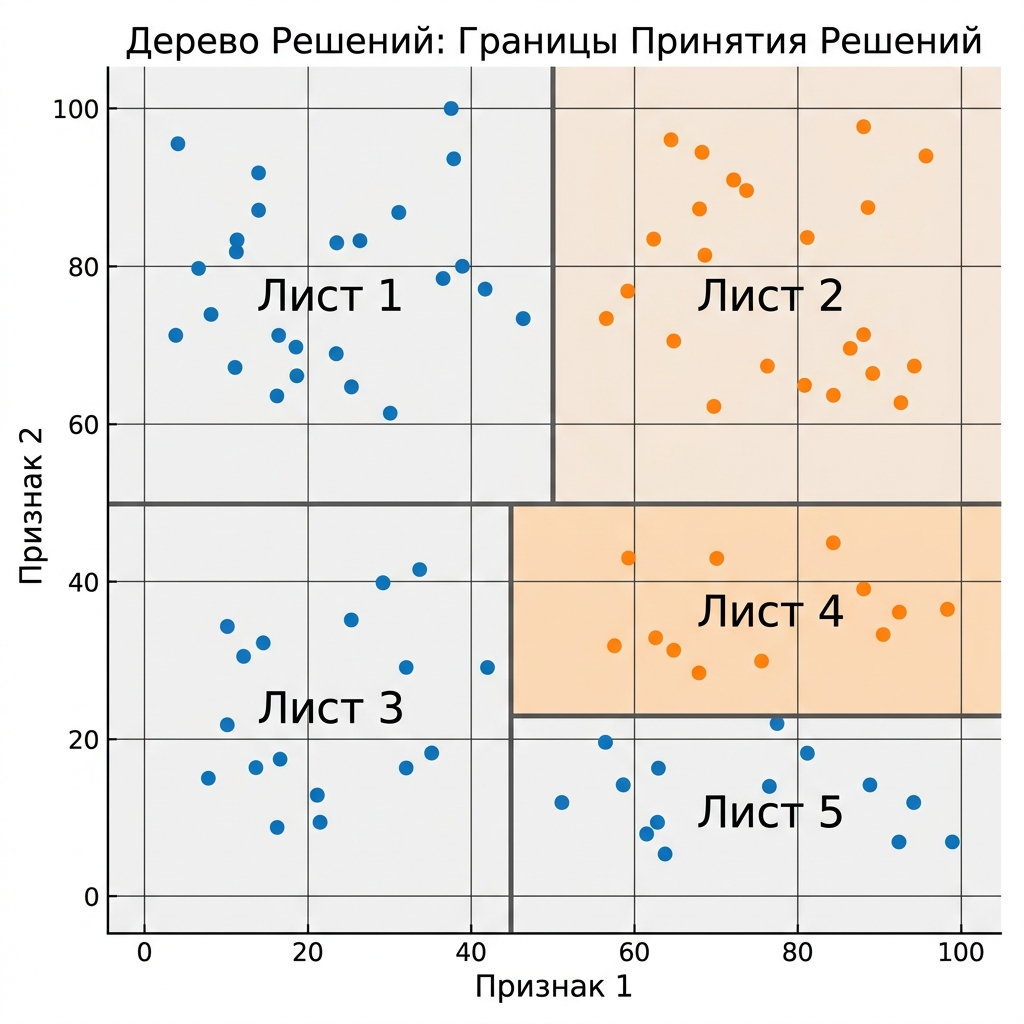
\includegraphics[width=0.30\textwidth]{tree_partition.png}
    \caption{Разбиение признакового пространства на гиперпрямоугольники (листы).}
\end{figure}

\commentary{Дерево — это отличный интерполятор, но плохой предсказатель «будущих рекордов». Оно никогда не предскажет цену квартиры выше, чем та, что была в обучении.}

\subsection{Жадный алгоритм построения}

\begin{itemize}
    \item \textbf{Вопрос}: Почему построение оптимального дерева — NP-трудная задача и в чем суть реализации «жадного» подхода?
    \item \textbf{Ответ}: Поиск глобально оптимального дерева требует перебора всех возможных структур и последовательностей разбиений. Количество таких вариантов растет как сверхэкспонента от числа признаков и объектов. 
    \item \textbf{Реализация (ID3, C4.5, CART)}: Используется алгоритм \textbf{рекурсивного разбиения} (Recursive Partitioning):
    \begin{enumerate}
        \item Начинаем с корневого узла, содержащего всю обучающую выборку $X$.
        \item В текущем узле перебираем все возможные пары (признак $j$, порог $t$).
        \item Для каждой пары вычисляем \textit{критерий информативности} (индикация того, насколько «чище» станут данные после сплита).
        \item Выбираем пару $(j, t)$, дающую максимальный выигрыш (\textbf{жадный выбор}).
        \item Разбиваем выборку на две части и рекурсивно повторяем шаги для дочерних узлов до срабатывания критериев остановки (остановка рекурсии).
    \end{enumerate}
\end{itemize}

\commentary{Жадность — это как выбор самого вкусного куска торта прямо сейчас вместо того, чтобы сесть на диету ради здоровья в будущем. Это работает быстро, но не гарантирует идеальный результат для всей структуры.}

\subsection{Критерии ветвления и информативность}

\begin{itemize}
    \item \textbf{Gain (Прирост информативности)}: $G(Q, j, t) = I(Q) - \frac{|Q_L|}{|Q|} I(Q_L) - \frac{|Q_R|}{|Q|} I(Q_R)$, где $Q$ — выборка в узле, $I$ — функция информативности. Мы максимизируем $G$, минимизируя взвешенную неопределенность в детях.
    
    \item \textbf{Классификация}:
    \begin{itemize}
        \item \textbf{Энтропия Шеннона}: $H(p) = -\sum p_k \log p_k$. Основана на теории информации. Более «чувствительна» к изменениям вероятностей классов, чем Джини, и стремится создавать максимально сбалансированные или идеально чистые узлы.
        \item \textbf{Критерий Джини}: $G = \sum p_k (1 - p_k) = 1 - \sum p_k^2$. Математически это вероятность ошибки при случайном выборе класса из распределения в узле. Джини вычислительно эффективнее (нет логарифмов) и чаще используется по умолчанию (например, в sklearn).
    \end{itemize}
    
    \item \textbf{Регрессия}:
    \begin{itemize}
        \item \textbf{MSE (Mean Squared Error)}: $I(Q) = \frac{1}{|Q|} \sum (y_i - \bar{y})^2$. Это дисперсия ответов. Минимизация MSE заставляет модель предсказывать среднее значение по листу. \textit{Почему хорошо?} Она математически удобна и сильно штрафует за большие отклонения.
        \item \textbf{MAE (Mean Absolute Error)}: $I(Q) = \frac{1}{|Q|} \sum |y_i - med(y)|$. Предсказывает медиану. \textit{Почему хорошо?} Она более устойчива (робастна) к выбросам в данных, чем MSE.
    \end{itemize}
\end{itemize}

\commentary{Критерий доли ошибок плох тем, что он «грубый» — он может не измениться после сплита, даже если классы стали более разделенными.}

\subsection{Работа с особенностями данных}

\begin{itemize}
    \item \textbf{Категориальные признаки}:
    \begin{itemize}
        \item \textbf{One-Hot Encoding}: Подходит для признаков с малой мощностью. Минус: сильно раздувает признаковое пространство и заставляет дерево делать много «неэффективных» сплитов.
        \item \textbf{Группировка по таргету (Метод CART)}: Категории сортируются по среднему значению целевой переменной (в случае регрессии или бинарной классификации). Это превращает категориальный признак в порядковый, и задача сводится к поиску порога $t$. Доказано, что для бинарной классификации и регрессии такой жадный поиск дает оптимальное разбиение среди всех возможных разбиений категорий на две группы.
    \end{itemize}
    
    \item \textbf{Пропущенные значения (Missing Values)}:
    \begin{itemize}
        \item \textbf{Направление по умолчанию}: Объект с пропуском отправляется в ту сторону, где ошибка на обучающей выборке была меньше, либо в сторону большинства объектов.
        \item \textbf{Суррогатные сплиты}: Если признак для основного сплита пропущен, используется «запасной» признак, который максимально коррелирует с основным (дает похожее разбиение выборки).
        \item \textbf{Отдельная категория}: Пропуск можно выделить в отдельное значение признака.
    \end{itemize}
\end{itemize}

\subsection{Регуляризация}

\begin{itemize}
    \item \textbf{Pre-pruning (Критерии остановки)}:
    \begin{itemize}
        \item \textbf{Max depth}: Ограничивает глубину, предотвращая создание слишком специфичных правил.
        \item \textbf{Min samples split/leaf}: Запрещает создавать узлы, в которые попадает слишком мало объектов. Это защищает от подстройки под шум.
        \item \textbf{Min impurity decrease}: Сплит делается только если он значимо уменьшает ошибку.
    \end{itemize}
    \item \textbf{Post-pruning (Стрижка)}:
    Позволяет дереву сначала «переобучиться» (построиться до конца), а затем удаляет узлы, которые не дают значимого прироста качества на валидации. Один из популярных методов — \textbf{Cost-Complexity Pruning} (минимизация функции $Loss + \alpha |Leaves|$).
\end{itemize}

\subsection{Алгоритмические оптимизации (Трюки)}

\begin{itemize}
    \item \textbf{Сортировка (Exact Greedy Algorithm)}:
    \begin{itemize}
        \item \textbf{Принцип}: Для каждого признака значения сортируются ($O(N \log N)$), после чего перебор всех возможных порогов занимает $O(N)$. Общая сложность поиска сплита: $O(D \cdot N \log N)$.
        \item \textbf{Плюсы}: Находит \textbf{идеальный порог}, обеспечивая максимальную точность для одного дерева.
        \item \textbf{Минусы/Сложность}: Огромное потребление памяти (нужно хранить отсортированные индексы для каждого признака). Плохо масштабируется на очень большие данные (миллионы строк).
    \end{itemize}
    
    \item \textbf{Гистограммный метод (Histogram-based Algorithm)}:
    \begin{itemize}
        \item \textbf{Принцип}: Значения признака разбиваются на $k$ корзин (бинов, обычно $k=256$). Вместо перебора всех значений $N$, перебираются только границы бинов. 
        \item \textbf{Плюсы}: 
            \begin{enumerate}
                \item \textbf{Скорость}: Поиск сплита занимает $O(D \cdot k)$ вместо $O(D \cdot N)$.
                \item \textbf{Память}: Данные можно хранить в `uint8` (номера бинов), что экономит до 4-8 раз больше места.
                \item \textbf{Subtraction Trick}: Гистограмму для большего ребенка можно получить вычитанием гистограммы меньшего ребенка из родительской ($O(k)$), что вдвое ускоряет расчеты.
            \end{enumerate}
        \item \textbf{Минусы}: Небольшая \textbf{потеря точности} из-за дискретизации (обычно нивелируется в ансамблях). Сложность реализации (нужно аккуратно обрабатывать границы и разреженные данные).
    \end{itemize}
\end{itemize}

\antigravity{Гистограммный метод — это "секретный соус" современных библиотек (LightGBM, CatBoost), позволяющий обучать деревья на миллионах строк за секунды.}

\end{document}
